\documentclass[11pt,a4paper]{article}
\usepackage[margin=23mm]{geometry}
\usepackage{fontspec}
\setmainfont{texgyrepagella}[Extension=.otf,UprightFont=*-regular,BoldFont=*-bold,ItalicFont=*-italic,BoldItalicFont=*-bolditalic]
\setsansfont{texgyreheros}[Extension=.otf,UprightFont=*-regular,BoldFont=*-bold,ItalicFont=*-italic,BoldItalicFont=*-bolditalic]
\usepackage{amsmath,amssymb,booktabs,graphicx,microtype,siunitx,tabularx,longtable,array,subcaption}
\usepackage{ragged2e}
\newcolumntype{P}[1]{>{\RaggedRight\arraybackslash}p{#1}}
\newcolumntype{Y}{>{\RaggedRight\arraybackslash}X}
\usepackage[numbers,sort&compress]{natbib}
\usepackage{xcolor}
\usepackage[hyphens]{url}
\usepackage{hyperref}
\usepackage[nameinlink]{cleveref}
\hypersetup{colorlinks=true,linkcolor=blue!45!black,citecolor=blue!45!black,urlcolor=blue!45!black,pdftitle={Additive Manufacturing of Molten Glass: Evidence, Physics and Engineering Roadmap}}
\setlength{\emergencystretch}{3em}
\setlength{\parskip}{0.35em}
\setlength{\parindent}{0pt}
\setlength{\tabcolsep}{4pt}
\renewcommand{\arraystretch}{1.18}
\newcommand{\NR}{\textit{NR}}
\title{Additive Manufacturing of Molten Glass\\\large Evidence, Process Physics, Hardware, and an Engineering Roadmap}
\author{Glass 3D Printing Research Project\\\small Technical evidence review and reproducible analysis}
\date{30 September 2026}
\begin{document}
\maketitle
\begin{abstract}
Molten-glass additive manufacturing connects glass chemistry, viscous flow, thermal history, motion planning, and defect-sensitive qualification. This review distinguishes reservoir extrusion and laser filament deposition from powder-bed processing and indirect composite routes. It synthesizes primary apparatus studies, manufacturer reference data, patent disclosures, and commercial evidence while making gaps in measurement explicit. Reproducible viscosity fits and flow/thermal scaling calculations explain process tradeoffs without presenting model scenarios as machine performance. A practical roadmap prioritizes feedstock identity, interlayer contact, temperature measurement, dimensional control, and end-use qualification. The accompanying archive includes source records, downloaded literature, figures, scripts, and the modular LaTeX project.
\end{abstract}
\textbf{Evidence status.} Initial sourcing occurred on 26 September 2026; targeted source verification continued on 29 September, with final editorial review on 30 September. This is a scoped technical review, not a certified exhaustive systematic review or a design certification. Missing specifications are reported as unknown. Calculated scenarios are identified separately from experimental findings.
\tableofcontents
\clearpage
\section{Introduction, scope, and process taxonomy}
\label{sec:introduction}
\subsection{The manufacturing question}
The useful question is not simply whether glass can be printed. It is whether a specified composition can be formed into an accepted geometry, at a repeatable rate, with the required optical, mechanical, thermal, and chemical properties. A transparent sculpture, a microfluidic channel, and a load-bearing glass connection place very different demands on the process. This report centers on direct deposition of hot inorganic glass and uses other additive routes as explicitly identified comparators.

The strongest case for additive manufacturing is geometric customization that is expensive or impractical with a repeated mold or accessible machining surface. Eliminating a mold does not eliminate conditioning, finishing, thermal treatment, or inspection. Conversely, accepting the native layer texture can create useful optical and aesthetic functions. Decisions should therefore begin with a part specification and a conventional-process baseline, not an assumption that additive manufacture is preferable.

\subsection{A taxonomy by material state and consolidation step}
\textbf{Reservoir-fed molten extrusion} conditions a quantity of glass in a crucible and deposits it through a heated nozzle. Gravity, imposed pressure, or mechanical metering drives flow. The receiving chamber manages cooling while a motion system lays down a continuous cord. Early G3DP and G3DP2 are reference demonstrations of this family.\cite{acad_klein2015,acad_inamura2018}

\textbf{Locally heated solid-feed deposition} delivers a glass rod or filament to a hot zone. A furnace-like nozzle or a laser heats only the material needed for deposition. Laser filament systems are particularly relevant to fused silica, whose viscosity at the same temperature differs greatly from soda-lime compositions. This route is analogous in material delivery to wire-fed directed-energy deposition, but it requires glass-specific treatment of optical absorption and stress.\cite{acad_liu2022}

\textbf{Powder-bed fusion} scans successive powder layers with a heat source. Packing, absorption, track consolidation, residual porosity, and cracking become central variables. Laser scan speed is not a net part-production rate: powder recoating, track overlap, contour passes, and rejected builds must be included. The labels SLS and SLM in the glass literature should be interpreted from the actual consolidation mechanism rather than treated as proof of complete densification.\cite{phys_datsiou}

\textbf{Indirect printing and conversion} shapes silica-containing inks, photopolymer nanocomposites, or precursors before drying, debinding, and densification. Stereolithography, two-photon polymerization, direct ink writing, and computed axial lithography belong here when the printed object is a precursor rather than final dense glass. The printing temperature can be near room temperature while subsequent firing is much hotter. Kotz and colleagues demonstrated transparent fused-silica structures by photopolymerizing a nanocomposite and heat treating it; Toombs and colleagues demonstrated volumetric shaping followed by sintering.\cite{phys_kotz,phys_toombs}

These routes exclude glass-fiber-filled thermoplastics, sugar glass, and metallic glasses from the core comparison. Chalcogenide glass extrusion is considered in the academic directory as a distinct material family, not as evidence for the same silicate processing window. Additively manufacturing a metal mold used to form glass is also an adjacent tooling route rather than direct glass printing.

\subsection{Evidence selection and reproducibility}
Source discovery covered primary journal articles, institutional repositories, manufacturer technical documents, institutional project pages, and patent records. DOI metadata were collected from Crossref where accessible; downloaded PDFs were parsed and retained with provenance. Reviews informed discovery but did not substitute for primary apparatus or property evidence. Institutional and manufacturer pages establish reported activity or supplier claims, not independently audited performance.

The companion source index and manifest retain individual records, retrieval dates, local paths, and asset hashes. Different versions of a supplier page were encountered during research; current certified ratings were not inferred from an older cached specification. Where a paper or site was blocked, the report identifies the narrower evidence actually available. This search did not enumerate every indexed paper or conduct a formal study-quality meta-analysis. Coverage of named institutions is an evidence map, including explicit negative search outcomes, rather than proof of their current equipment inventories.

Table~\ref{tab:routes} is deliberately a comparison of documented examples. It is not a normalized benchmark. NR means that the cited evidence does not establish a comparable numerical value; it does not mean zero or poor performance. Relative tensile strength is particularly unsuitable for inference from bend tests performed on different compositions and flaw populations.

\begin{table}[htbp]
\centering\small
\caption{Direct molten extrusion versus powder-bed fusion and photopolymer/sintering routes. Temperatures and rates refer to the indicated examples, not universal or certified machine limits.}
\label{tab:routes}
\begin{tabularx}{\textwidth}{@{}P{0.17\textwidth}YYY@{}}
\toprule
Metric & Molten reservoir extrusion & Glass laser powder-bed fusion & Photopolymer shaping + sintering \\
\midrule
Representative evidence & G3DP2, 2018 \cite{acad_inamura2018} & Soda-lime LPBF, 2019 \cite{phys_datsiou} & Fused-silica SLA, 2017; micro-CAL, 2022 \cite{phys_kotz,phys_toombs} \\
Temperature ($^{\circ}$C) & Reservoir operating 1090; separate delivery/build zones & Local transient melt temperature NR; 1280 is the paper's material thermal-characterization value, not a measured laser-pool setpoint & Near-ambient shaping; formulation-specific high-temperature densification. UpQuartz example: 1300 sintering \cite{com_upnano} \\
Build envelope & G3DP2: $320\times320\times350$ mm; earlier G3DP: $250\times250\times300$ mm (source Table~1) & Comparable validated maximum NR & Comparable validated maximum NR; demonstrated microstructures are not machine envelope \\
Deposition rate & G3DP2: 5.2 kg/h $\approx86.7$ g/min; deposited flow, excludes annealing & Net accepted-part rate NR & Net glass volume/time NR; micro-CAL exposure 30--90 s excludes subsequent firing \\
Optical transmission $T\%$ & Transparent demonstrators; comparable spectral $T\%$ NR & Opaque as-built examples; comparable spectral $T\%$ NR & Transparent fused silica reported; comparable thickness/wavelength-normalized $T\%$ NR \\
Surface roughness $R_a$ & Comparable quantified $R_a$ NR; bead texture retained & Comparable quantified $R_a$ NR; partially fused surface particles & Micro-CAL sintered lens: $R_a=60$ nm over 523 $\mu$m; 6 nm over 49 $\mu$m (source Fig.~S17); not a whole-part specification \\
Relative tensile strength & NR: bending/structural tests cannot establish a universal tensile ratio & NR & NR: specimen type and loading differ \\
\bottomrule
\end{tabularx}
\end{table}

The G3DP2 paper reports both 570 mm$^3$/s and 5.2 kg/h as rounded production descriptors; neither includes a complete end-to-end production cycle. Its comparison to earlier platforms should not be extended to every modern indirect printer. The LPBF study reported approximately 11--12\% internal porosity in selected specimens and observed improved translucency with a subsequent 650~$^{\circ}$C heat treatment. Those findings concern one powder and processing window, not an upper bound on all powder-bed glass methods.\cite{acad_inamura2018,phys_datsiou}

\begin{figure}[htbp]
\centering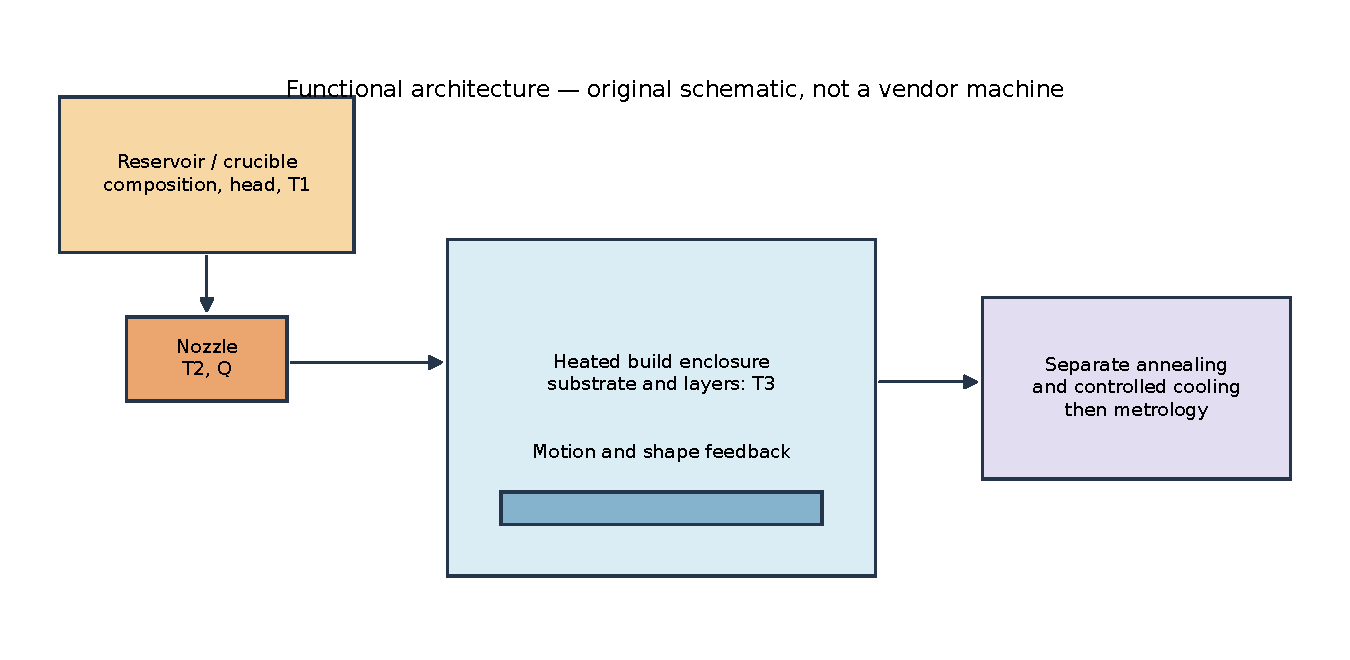
\includegraphics[width=\linewidth]{figures/process_architecture.pdf}
\caption{Original functional schematic separating reservoir conditioning, delivery, receiving environment, and downstream annealing. It describes engineering functions, not the construction or specification of a particular commercial printer.}
\label{fig:architecture}
\end{figure}

\section{Rheology, thermal properties, and material physics}
\label{sec:physics}
\subsection{A glass name is not a constitutive law}
Composition, hydroxyl content, impurities, and thermal history influence the response of glass. ``Borosilicate'' and ``soda-lime'' identify families rather than unique viscosity curves. Fused quartz and synthetic fused silica are also not automatically interchangeable grades. Accordingly, the calculations below use three named manufacturer products as reference materials: SCHOTT AR-GLAS, SCHOTT BOROFLOAT 33, and Corning HPFS 7980. They are not asserted to be the feedstocks used by the cited printers.\cite{phys_ar,phys_boro,phys_silica}

\subsection{Viscosity law, units, and fitting method}
Write the Vogel--Fulcher--Tammann form as
\begin{equation}
 y=\log_{10}\!\left[\frac{\eta}{1\,\mathrm{dPa\,s}}\right]
 =A+\frac{B}{T_C-T_{0,C}},\qquad
 T_C=T_{0,C}+\frac{B}{y-A}.
\label{eq:vft}
\end{equation}
Here $T_C$ and $T_{0,C}$ use degrees Celsius consistently, while their difference and $B$ have kelvin units. Changing the temperature origin requires shifting $T_0$ by the same amount. Since $1\,\mathrm{dPa\,s}=0.1\,\mathrm{Pa\,s}$, the logarithm expressed in Pa\,s is $y-1$. A numerical viscosity must always be associated with its unit before use in a flow equation.

The AR-GLAS curve fits three nominal points: 530, 720, and 1040~$^{\circ}$C at $y=13$, 7.6, and 4. The BOROFLOAT curve fits four points, adding the 518~$^{\circ}$C strain point to its 560, 820, and 1270~$^{\circ}$C annealing, softening, and working points. Nonlinear least squares fits $A$, $B$, and $T_0$ in logarithmic viscosity. There is no statistical uncertainty claim: the source values are nominal property anchors, not a replicated experimental dataset.\cite{phys_ar,phys_boro}

For HPFS 7980, an Arrhenius approximation fixes $T_{0,K}=0$, equivalently $T_{0,C}=-273.15$, and fits $A+B/T_K$ to the manufacturer's three reference points. This is a constrained limiting form of VFT used to illustrate a strong-glass response; it is an analyst-selected approximation, not a Corning-provided constitutive law. The listed strain, annealing, and softening points are 893, 1042, and 1585~$^{\circ}$C. The resulting fit does not reproduce them exactly.\cite{phys_silica}

\begin{table}[htbp]\centering\small
\caption*{Computed fit parameters. Temperature origin is Celsius in Equation~\ref{eq:vft}. RMS refers to residuals in $\log_{10}(\mathrm{dPa\,s})$, not measurement uncertainty.}
\begin{tabular}{lrrrr}
\toprule Material & $A$ & $B$ (K) & $T_{0,C}$ & RMS \\
\midrule
AR-GLAS & -1.89655 & 4977.503 & 195.862 & $<10^{-12}$ \\
BOROFLOAT 33 & -1.68081 & 6578.032 & 111.631 & 0.00655 \\
HPFS 7980, constrained & -4.16293 & 22072.095 & -273.150 & 0.27547 \\
\bottomrule\end{tabular}
\end{table}

The near-zero AR-GLAS residual is a consequence of fitting three parameters to three anchors; it is not evidence of exceptionally accurate prediction. The silica fit's largest residual is about 0.38 decades, a factor of roughly 2.4 in viscosity. A temperature inferred from that curve must not replace a manufacturer's annealing point or an independently measured rheology dataset. A fitted interval is shown separately from extrapolation in Figure~\ref{fig:vft}.

\begin{figure}[htbp]\centering
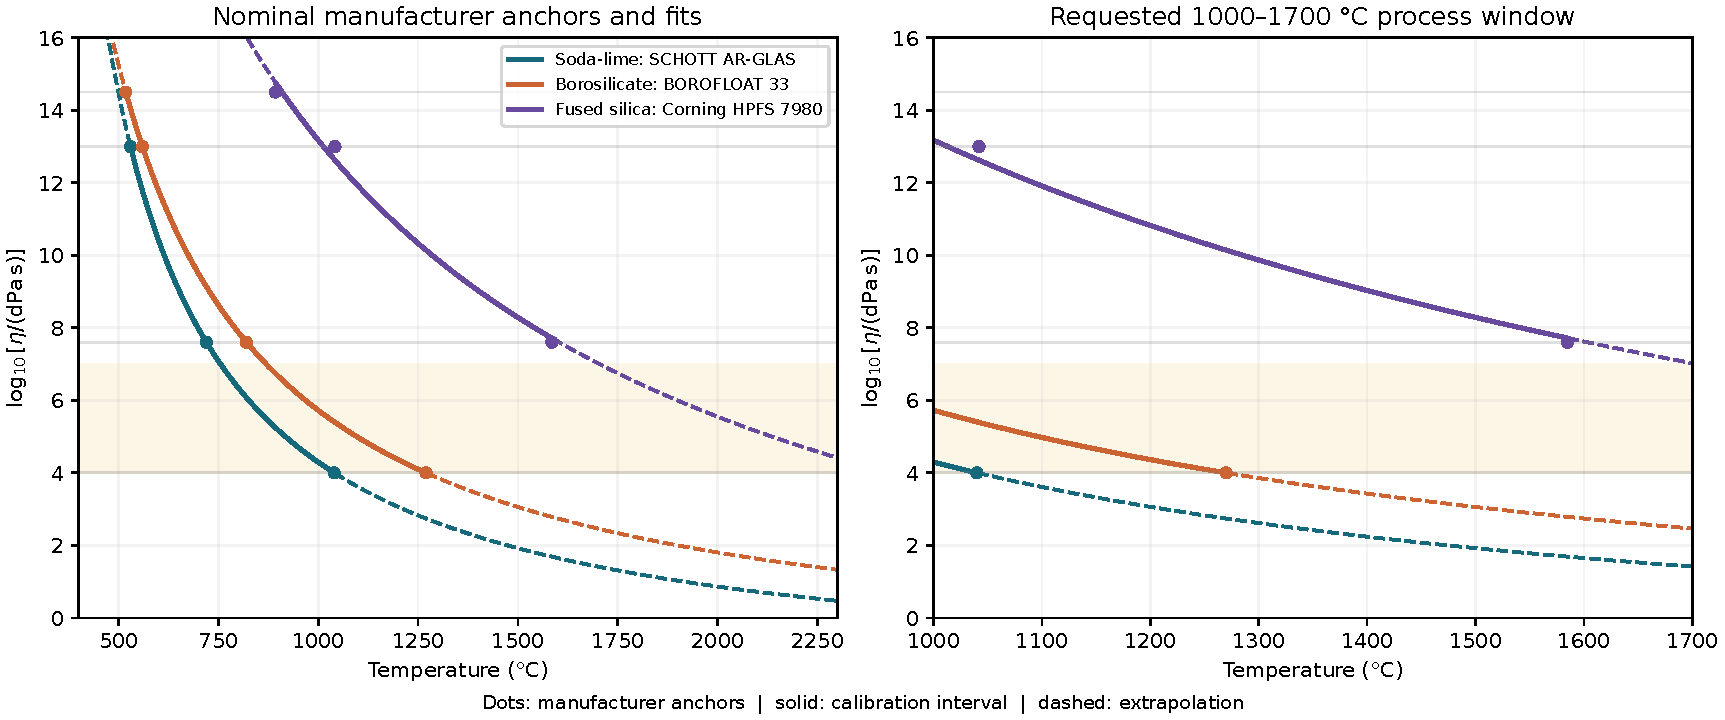
\includegraphics[width=\linewidth]{figures/viscosity_vft.pdf}
\caption{Calculated viscosity curves from nominal, composition-specific manufacturer reference points. Solid segments lie between the lowest and highest fitting anchors; dashed segments are extrapolation. The shaded $10^4$--$10^7$ dPa\,s band is a descriptive working band for comparison, not a validated universal printing window. HPFS uses the approximate constrained model described in the text.}
\label{fig:vft}\end{figure}

\begin{table}[htbp]\centering\small
\caption*{Temperatures ($^{\circ}$C) obtained by inversion of the fitted curves, deliberately distinguished from reported manufacturer points. Columns correspond to $y=14.5$, 13, 7.6, and 4. The AR-GLAS strain estimate and silica working estimate are extrapolations; the silica softening estimate slightly exceeds its calibration interval.}
\begin{tabular}{lrrrr}\toprule Material & Strain & Annealing & Softening & Working \\ \midrule
AR-GLAS & 499.4 & 530.0 & 720.0 & 1040.0 \\
BOROFLOAT 33 & 518.2 & 559.7 & 820.4 & 1269.6 \\
HPFS 7980 (approx.) & 909.5 & 1012.9 & 1603.3 & 2430.8 \\
\bottomrule\end{tabular}

\end{table}

The computed HPFS working point near 2431~$^{\circ}$C is far outside the fitted data and should be treated only as an illustration of extrapolation risk. It is not a process recommendation: evaporation, optical absorption, and equipment/material limits require separate treatment. Even the 1000--1700~$^{\circ}$C plot contains substantial extrapolation for AR-GLAS. Publishing a smooth curve does not establish its validity throughout its axis range.

\begin{figure}[htbp]\centering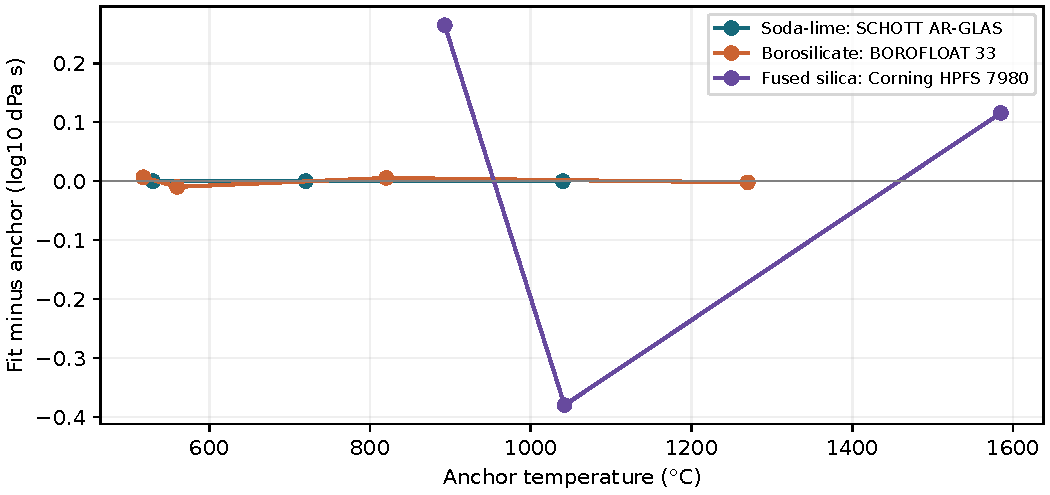
\includegraphics[width=.77\linewidth]{figures/viscosity_residuals.pdf}
\caption{Residuals reveal the approximation that a visually smooth curve can hide. The silica model is least suitable for selecting annealing setpoints. Manufacturer reference points should be retained as reported rather than silently replaced with fitted values.}
\end{figure}

\subsection{Flow, capillarity, and a worked scaling example}
For a cord radius $r$, speed $U$, density $\rho$, surface tension $\gamma$, and dynamic viscosity $\eta$, useful ratios are
\begin{equation}
 \mathrm{Re}_d=\frac{2\rho Ur}{\eta},\quad
 \mathrm{Ca}=\frac{\eta U}{\gamma},\quad
 \mathrm{Bo}_r=\frac{\rho gr^2}{\gamma},\quad
 \mathrm{Oh}_r=\frac{\eta}{\sqrt{\rho\gamma r}}.
\end{equation}
The subscripts explicitly identify the length convention; radius-based and diameter-based definitions differ. Very small Reynolds number does not mean that gravity or surface tension is negligible. It means that inertia is small relative to viscous stresses under the assumed scale.

Consider a hypothetical isothermal cylindrical nozzle with radius 5 mm, length 10 mm, melt head 0.2 m, $\rho=2500$ kg/m$^3$, $\eta=1000$ Pa\,s, and assumed $\gamma=0.3$ N/m. These are scenario inputs, not a commercial specification. Equation~\ref{eq:nozzleflow} predicts a pressure of 4905 Pa, $Q=1.204\times10^{-7}$ m$^3$/s, and 1.083 kg/h. The mean nozzle speed is 1.533 mm/s. Using that speed gives $\mathrm{Re}_d=3.83\times10^{-5}$, $\mathrm{Ca}=5.11$, $\mathrm{Bo}_r=2.04$, and $\mathrm{Oh}_r=516$. This low-inertia example is sensitive to viscosity and radius; its short nozzle also makes entrance effects a material omission. It does not predict actual accepted-part throughput.

\begin{figure}[htbp]\centering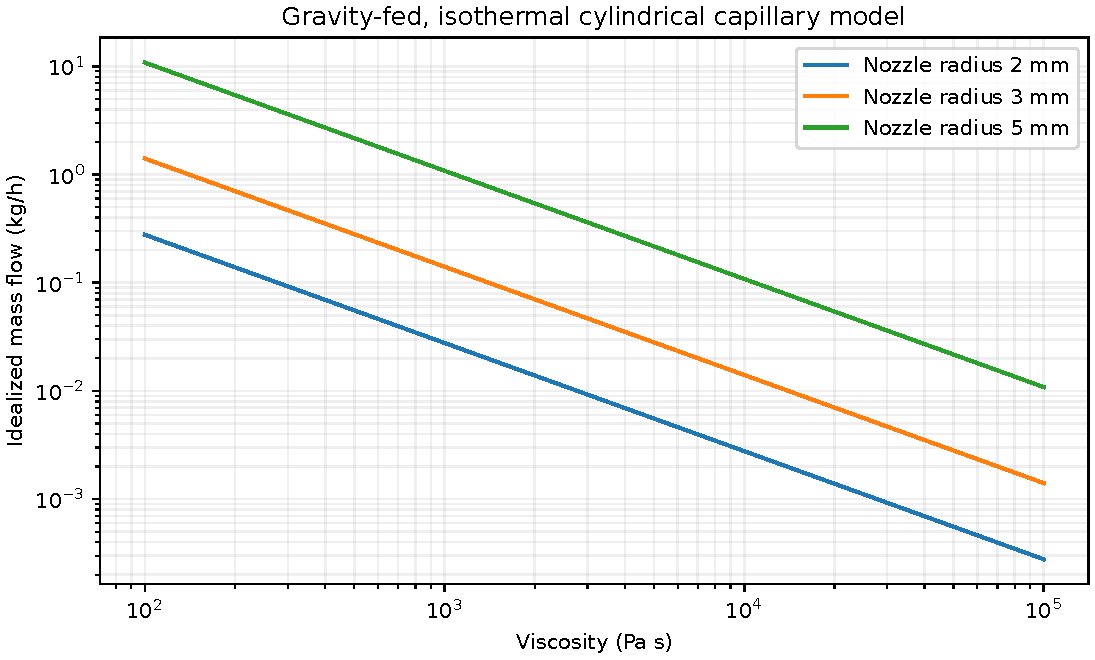
\includegraphics[width=.83\linewidth]{figures/flow_sensitivity.pdf}
\caption{Scenario calculation for a 0.2 m head, 10 mm bore length, and assumed constant density. The $r^4/\eta$ dependence explains why thermal drift and nozzle wear are important. No measured machine performance is plotted.}
\end{figure}

The local viscosity sensitivity follows directly from the fit:
\begin{equation}
 \frac{\mathrm{d}\ln\eta}{\mathrm{d}T}=-\ln(10)\frac{B}{(T-T_0)^2},\qquad
 \frac{\mathrm{d}\ln Q}{\mathrm{d}T}\simeq-\frac{\mathrm{d}\ln\eta}{\mathrm{d}T}.
\end{equation}
The second relation holds only when the other capillary-model inputs remain fixed. It motivates temperature feedback without implying that a heater command controls glass temperature instantaneously.

\subsection{Instability, slumping, and interlayer contact}
For an ideal inviscid free cylindrical jet in a dynamically negligible exterior fluid, the fastest growing axisymmetric capillary mode has wavelength approximately $9.02r=4.51d$. That familiar Rayleigh result is not a universal optimum for a viscous glass bead contacting a substrate. Viscosity contrast, cooling, stretching, finite length, contact angle, and the receiving surface change the instability problem; Tomotika's viscous-thread treatment illustrates the importance of the surrounding fluid.\cite{phys_rayleigh,phys_tomotika}

The viscous capillary scale $t_\gamma\sim\eta r/\gamma$ is about 16.7 s for the preceding scenario. A gravitational deformation scale $t_g\sim\eta/(\rho gH)$ is about 0.41 s for an assumed unsupported height $H=0.1$ m. These order-of-magnitude times refer to a material that remains at the selected viscosity. A rapidly cooling, attached bead violates that assumption, and neither value is an observed failure time. They show why shape arrest and bonding must be controlled together.

Surface-tension gradients can impose tangential stresses, $\eta\,\partial u_t/\partial n\sim\partial\gamma/\partial s$. Temperature and composition variations can therefore drive Marangoni flow even when bulk inertia is small. Quantifying it requires the actual derivative of surface tension and local thermal field; a generic sign or magnitude is not assigned here. Similarly, capillary neck growth between adjacent beads is only one contribution to adhesion. Contact area, surface contamination, and the time-temperature history must accompany any comparison of interlayer strength.

\subsection{Thermal scales and materials outside the fitted set}
Using BOROFLOAT's reference $k=1.2$ W/(m K) at 90~$^{\circ}$C, $c_p=830$ J/(kg K) over 20--100~$^{\circ}$C, and nominal density 2230 kg/m$^3$ gives an approximate low-temperature diffusivity $a\approx6.48\times10^{-7}$ m$^2$/s. Characteristic diffusion times $L^2/a$ are approximately 39 s at $L=5$ mm and 617 s at 20 mm. These are scaling calculations using low-temperature reference properties, not high-temperature annealing schedules. Radiation, temperature-dependent properties, and boundary conditions become significant in a real print.\cite{phys_boro}

Aluminosilicates add a broad composition space with varying modifiers, liquidus behavior, and viscosity. No single aluminosilicate curve is defensibly inferred from the three products above. A useful extension would specify a grade and obtain measured viscosity, expansion, crystallization kinetics, and compatible wet-contact materials before fitting. This explicit gap is preferable to assigning plausible-looking coefficients to an unspecified composition.

\section{Nozzle mechanics, hardware, and kinematics}
\label{sec:hardware}
\subsection{Two materially different ways to deliver hot glass}
Reservoir extrusion and laser-heated filament deposition solve different hardware problems. In the former, a crucible provides an inventory of conditioned melt and a nozzle meters a continuous cord. In the latter, a solid feedstock carries material to a small hot zone; deposition occurs after local softening or melting. Separating these architectures prevents an inappropriate comparison between a furnace setpoint and a laser's nominal power. Both are direct hot-glass routes, but their thermal inventory, material residence time, attainable feature size, and interruption behavior differ.

The historical MIT G3DP apparatus demonstrated transparent reservoir-fed material extrusion with a heated receiving chamber. Its institutional project description specifies an upper kiln cartridge and a lower annealing chamber. The later G3DP2 paper describes three-zone thermal control and four-axis motion, alongside a demonstration of assembled architectural columns. These publications establish feasibility and increasingly integrated process control; they do not establish that every printed component is suitable for structural service without qualification.\cite{acad_klein2015,acad_mitproject,acad_inamura2018}

\subsection{Flow resistance and nozzle selection}
As a deliberately simplified design model, steady Newtonian flow through an isothermal cylindrical bore gives
\begin{equation}
 Q=\frac{\pi r^4}{8\eta L}\Delta p,\qquad
 \Delta p\simeq \rho g H+\Delta p_{\mathrm{act}},
 \label{eq:nozzleflow}
\end{equation}
where $r$ is bore radius, $L$ is bore length, $H$ is melt head, and $\Delta p_{\mathrm{act}}$ is any imposed pressure. The expression excludes entrance losses, capillary pressure, temperature gradients, slip, and a partially obstructed outlet. It should be treated as a scaling law for engineering estimates, not as a calibrated G3DP flow model. Its useful implications are immediate: doubling radius increases predicted flow sixteenfold; doubling viscosity halves predicted flow; and emptying a gravity-fed reservoir changes output even when the heater setpoint stays fixed.

For a slowly varying nozzle profile the corresponding approximation is
\begin{equation}
 \Delta p_{\mathrm{visc}}=\frac{8Q}{\pi}
 \int_0^L\frac{\eta[T(z)]}{r(z)^4}\,\mathrm{d}z.
\end{equation}
The coldest narrow section can therefore dominate pressure loss. A heater mounted above the tip cannot by itself prove that the issuing glass has the intended viscosity. A practical experimental calibration would weigh deposited glass against time while recording head height, nozzle temperatures, dwell time, and glass batch. A flow map should include warm-up and restart transients rather than only the best steady segment. This calibration protocol is a proposal of this review.

Refractory ceramic and precious-metal wet-contact parts require different qualification. MIT's historical project page uses the wording alumina--zircon--silica for its nozzle; that description should not be generalized to all apparatus versions. Heraeus documents platinum and platinum-alloy glass-manufacturing components and emphasizes that alloy choice depends on the glass and required purity. In particular, its optical-glass guidance favors rhodium-free platinum materials where coloration matters, while Pt--Rh alloys appear in other demanding glass-processing applications. Thus ``platinum--rhodium is always best'' is not a supportable design rule. Supplier information is evidence of materials availability and engineering considerations, not independent proof of a particular printer's nozzle life.\cite{acad_mitproject,acad_heraeus}

\subsection{Motion control is also material control}
Ignoring shrinkage and evaporation, conservation of mass relates deposited area $A_b$ to travel speed $U$ through $A_b\simeq Q/U$. A corner slowdown therefore increases local cross-section unless flow changes at the same time. Conversely, acceleration can thin a bead and reduce contact with the previous layer. Discontinuous paths add a second problem: molten glass stored downstream of a metering mechanism can continue moving after its command stops. Designing a path as a continuous loop reduces repeated starts, although it restricts accessible topology.

These observations motivate a proposed controller with separate estimation of thermal state, material delivery, and position. A geometric planner should specify the desired cross-section and contact location; a deposition controller should translate these into speed and flow commands with actuator delays. The controller should monitor actual bead shape rather than interpreting successful motor motion as successful deposition. Height feedback is particularly valuable because small layer errors accumulate and change the physical gap between nozzle or hot zone and the growing part.

Laser filament systems remove the need for a large nozzle filled with molten silica. Von Witzendorff and colleagues demonstrated quartz-fiber deposition using a CO$_2$ laser and translating substrate. Liu and colleagues subsequently examined symmetric laser heating and bonding of approximately $196\,\mu$m fused-silica filament; their multilayer experiment used $200\,\mu$m nominal layers. These are research operating conditions, not a universal printer resolution.\cite{acad_witzendorff2018,acad_liu2022} Their significance is that energy delivery, filament feed, and substrate motion jointly determine fusion. Nominal laser power alone cannot specify the delivered energy density without optical coupling, beam geometry, feedstock diameter, and speed.

\subsection{Proposed hardware qualification sequence}
\begin{figure}[htbp]
\centering
\begin{subfigure}[c]{.40\linewidth}\centering
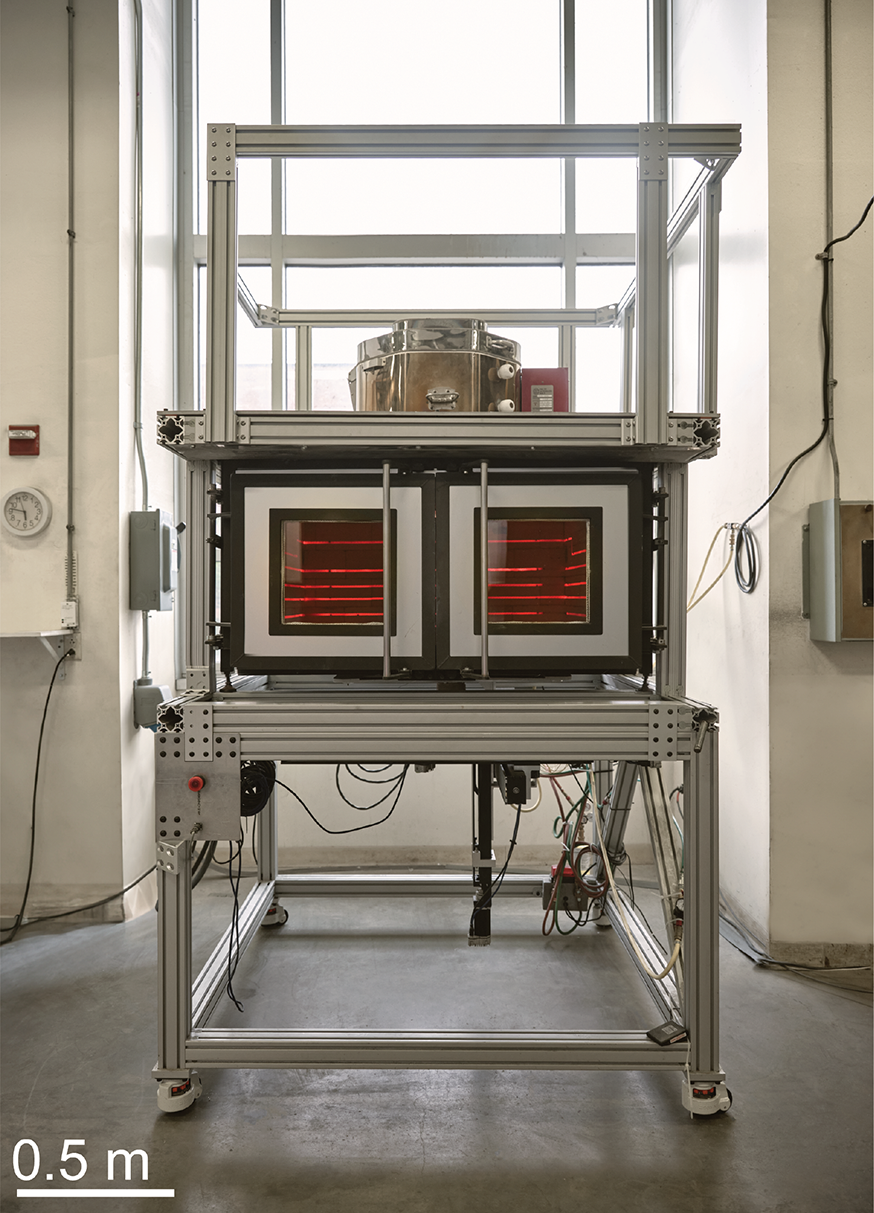
\includegraphics[height=62mm]{figures/Massimino2024_Figure1.png}
\caption{G3DP3 reservoir-fed apparatus.}
\end{subfigure}\hfill
\begin{subfigure}[c]{.55\linewidth}\centering
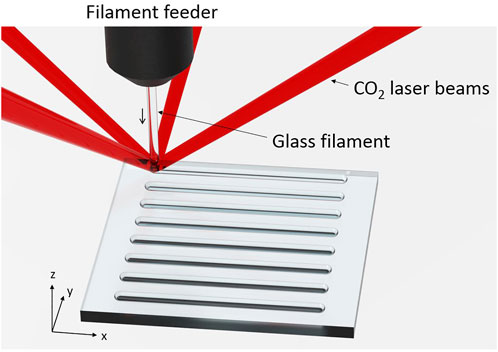
\includegraphics[width=\linewidth]{figures/Liu2022_Figure1.jpg}
\caption{Four-beam laser filament heating.}
\end{subfigure}
\caption{Contrasting thermal architectures. Left: Massimino et al. (2024), Figure 1, showing the G3DP3 build chamber below the furnace/crucible, \href{https://doi.org/10.1007/s40940-024-00279-8}{original article}. Right: Liu, Oriekhov and Fokine (2022), Figure 1, \href{https://doi.org/10.3389/fmats.2022.978861}{original article}. Both images reproduced unmodified under \href{https://creativecommons.org/licenses/by/4.0/}{CC BY 4.0}. The drawing and photograph are not to a common scale.}
\end{figure}
A useful acceptance sequence begins with stationary thermal characterization, proceeds to single tracks and starts/stops, then to turns, stacked walls, and representative enclosed geometries. At each stage, assess both geometric error and material integrity. For nozzles, inspect bore growth, adhering deposits, inclusions in the glass, and leakage at joints. For filament systems, inspect diameter variation, feed damage, and direction-dependent heating. These tests are recommended engineering controls rather than published capability claims. They make a machine specification reproducible: a build envelope without its hot-zone clearances, thermal stability, and supported path geometry is an incomplete description of usable manufacturing capacity.

\section{In-situ thermal management and annealing}
\label{sec:thermal}
\subsection{Deposition temperature and annealing temperature serve different purposes}
Hot-glass printing must establish intimate contact at a new interface while preserving the geometry already deposited. Heating promotes flow and bonding but also allows deformation; cooling arrests geometry but develops gradients and eventually freezes stress. A heated build chamber consequently addresses only part of the problem. It does not automatically certify completion of annealing, and a chamber thermocouple does not directly measure the coldest or hottest point inside a thick section.

G3DP2's separated thermal zones demonstrate an architecture that can manage melt preparation, delivery, and the receiving environment independently.\cite{acad_inamura2018} At smaller scales, Chen and colleagues report a closed-loop system adjusting CO$_2$ laser power from measured melt-zone temperature. Their quartz-glass experiments compare temperature-controlled deposition with constant-power cases and report improved formation quality. The paper supports feedback as an experimentally tested route; it does not establish that its sensor calibration, controller gains, or power limits transfer to another glass or optical arrangement. The article appeared online in December 2024 in the 2025 journal issue.\cite{acad_chen2025}

\subsection{A thermal model with explicit boundary assumptions}
For a continuum model with no internal chemical heat release, the local energy balance is
\begin{equation}
 \rho c_p(T)\left(\frac{\partial T}{\partial t}+\mathbf{u}\cdot\nabla T\right)
 =\nabla\cdot\left(k(T)\nabla T\right)+q_{\mathrm{abs}}.
 \label{eq:thermaltransport}
\end{equation}
Here $q_{\mathrm{abs}}$ represents absorbed volumetric heating. A solid or nearly arrested region can use $\mathbf{u}=0$; a flowing cord generally cannot. A common opaque-surface approximation is
\begin{equation}
 -k\nabla T\cdot\mathbf{n}
 =h(T-T_\infty)+\epsilon\sigma_{\mathrm{SB}}(T^4-T_{\mathrm{sur}}^4)-q''_{\mathrm{laser}}.
\end{equation}
All fourth-power temperatures must be in kelvin. Surface and volumetric laser absorption are alternative idealizations and must not count the same energy twice. Semitransparent glass may require spectral radiative transfer rather than an opaque gray surface. Contact with the substrate introduces another uncertain boundary: real conductance depends on wetting, interface area, and local conformity.

The dimensionless numbers
\begin{equation}
 \mathrm{Bi}=\frac{hL_c}{k},\qquad
 \mathrm{Fo}=\frac{a t}{L_c^2},\qquad a=\frac{k}{\rho c_p}
\end{equation}
provide a first check on model selection. A small convective Biot number favors a lumped-temperature approximation, but radiation and contact losses must also be included before invoking that approximation. The diffusion time $t_d\sim L_c^2/a$ explains why the thickest thermal section often matters more than total height. Doubling a conduction distance multiplies this time estimate by four for unchanged properties and boundary conditions. These equations are engineering models presented for interpretation; this review does not claim a validated three-dimensional simulation of any cited printer.

\subsection{Stress relaxation and cooling history}
SCHOTT's technical guidance identifies annealing conditions, glass type, size, and geometry as determinants of residual stress. Its conventional upper annealing and strain-point viscosities are $10^{13}$ and $10^{14.5}$ dPa\,s, respectively, equivalent to $10^{12}$ and $10^{13.5}$ Pa\,s. Confusing these units shifts a viscosity curve by one decade. Fine annealing involves temperature equalization and controlled cooling through the relevant relaxation range; rapid cooling farther below that range can still cause damaging temporary stress.\cite{acad_schott2023}

For interpretation, a Maxwell estimate gives a stress-relaxation time $\tau_M\sim\eta/G$, where $G$ is an appropriate shear modulus. The ratio $\tau_M/t_{\mathrm{process}}$ compares relaxation with the imposed thermal history. It is not a universal annealing recipe: real glass exhibits a relaxation spectrum and structural history dependence. Likewise, the restrained elastic estimate
\begin{equation}
 \sigma_{\mathrm{th}}\sim\frac{E\alpha_T\Delta T}{1-\nu}
\end{equation}
is a scale for stress magnitude, with coefficient depending on constraint and geometry. It must not be inserted as an exact residual-stress prediction for a free, three-dimensional print. Mechanical equilibrium, free surfaces, and viscoelastic relaxation determine the actual stress field.

\subsection{A proposed measurement-driven annealing workflow}
A defensible qualification program would first measure or obtain the specific batch's transition, expansion, and relaxation characteristics. Next, instrument a representative thick-section surrogate to estimate how chamber readings relate to internal temperature. Use that information to propose a dwell and cooling program, and verify the resulting parts by calibrated stress measurement and dimensional inspection. A hollow wall, solid base, and junction may require different local interpretation even within one object.

For thermal imaging, record spectral band, viewing geometry, reflected surroundings, assumed emissivity, and calibration method. A visually stable thermal image is not evidence of an accurate absolute temperature if the camera sees transmitted or reflected radiation. Recycled-glass printing work by Stern and colleagues explicitly investigated glass-dependent viscosity and used infrared thermography during extrusion, emphasizing why changing feedstock requires renewed process characterization.\cite{acad_stern2024}

In-situ heating and a separate annealing furnace should therefore be evaluated as a complete production schedule. Include transfer delays, loading orientation, furnace occupancy, and the slowest qualified cooling step when estimating throughput. A continuous lehr is a possible industrial design, but its residence-time distribution and compatibility with individually printed geometries would need demonstration. No operating continuous annealing lehr is inferred from the mere presence of a heated build chamber in the cited prototypes.

\section{Defect mechanisms and optical quality}
\label{sec:defects}
\subsection{A transparent object is not necessarily an imaging optic}
Optical qualification should separate total transmission, directional transmission, wavefront quality, and scattering. A ribbed transparent wall can transmit considerable light while producing strong image distortion. Conversely, a deliberately patterned illumination element may use that distortion productively. The early G3DP work demonstrates transparent structures and controllable caustic patterns; it is not evidence that an as-printed wall has the surface figure of a polished lens.\cite{acad_klein2015}

Destino and colleagues provide a different benchmark: silica and silica--titania glasses prepared by sol--gel-derived ink writing followed by thermal processing were characterized against commercial optical glasses. Their work includes polished surfaces and refractive-index homogeneity, so those results should not be attributed to as-deposited molten cords.\cite{acad_destino2018} Cross-route comparisons need the whole process history, including polishing, thermal densification, coatings, and measurement path length.

\subsection{Mechanism-based diagnosis}
Entrained gas, inter-track voids, crystalline inclusions, foreign particles, and surface damage can all reduce performance but demand different remedies. Gas already in a reservoir calls for feedstock and conditioning investigation. Voids recurring at junctions suggest deposition geometry or insufficient bonding. A rough surface can arise from layer shape without implying bulk porosity. Crystals require phase-sensitive characterization; their presence must not be inferred from every bright spot in a microscope image.

Devitrification depends on composition, nucleation sites, temperature, and exposure time. A liquidus temperature describes an equilibrium phase boundary, not a complete kinetic guarantee that a print remains amorphous. Recommended characterization includes differential scanning calorimetry at stated heating rates, diffraction, and microscopy after representative thermal cycles. Recycling further demands chemical identity and contamination checks. Mixing individually transparent cullets does not establish thermal compatibility or a common viscosity curve. These are proposed qualification measures, not claims that the cited recycled-glass study demonstrated every test.

For optical loss, a basic homogeneous attenuation model is
\begin{equation}
 T_{\mathrm{int}}(\lambda,d)=\exp[-\mu(\lambda)d].
\end{equation}
External transmission also includes interface reflections, collection geometry, and scattering. For a simple plane-parallel transparent specimen, surface reflection losses cannot be silently assigned to bulk absorption. Reporting a single percentage without wavelength, thickness, surface condition, and whether scattered light is collected is insufficient for ranking processes. Likewise, roughness $R_a$ is a profile statistic at a stated cutoff and direction; it does not alone specify optical wavefront quality.

\subsection{Interlayer bonding and mechanical evidence}
The KTH filament study measured both line geometry and bonding width, providing evidence that deposited width and actual contact width need not be equal. Its multilayer results demonstrate reproducible bonding under the selected operating conditions, not an independently measured universal tensile strength.\cite{acad_liu2022} A visible line in a transparent print may represent surface geometry, an internal interface, compositional variation, or stress; fracture analysis is needed to identify the feature that actually controls failure.

A 2026 study by Chhadeh and colleagues directly addresses mechanical performance of extruded soda-lime glass. Its four-point bending experiments show dependence on toolpath and layer orientation and connect performance to thermal retention during deposition. The reported $90^\circ$ specimens had mean strength approximately 40\% greater than the $0^\circ$ specimens in that experiment. This is a within-study comparison, not a transferable design factor. The test setup deliberately differs from EN~1288-3 in dimensions and roller freedom; it should not be described as unqualified standard conformity.\cite{acad_chhadeh2026}

The engineering implication is that orientation labels alone are inadequate predictors: they can also change path length, return time, and the heat history of adjacent tracks. A proposed experimental design should hold those factors separately where possible and record specimen surface treatment, effective loaded area, loading rate, environment, and failure origin. Report the specimen count and full strength distribution rather than the strongest coupon. Comparing flexural strength with direct tensile strength, or comparing specimens with different flaw populations, can obscure the actual process improvement.

\subsection{Polarimetry and an application-specific acceptance chain}
\begin{figure}[htbp]\centering
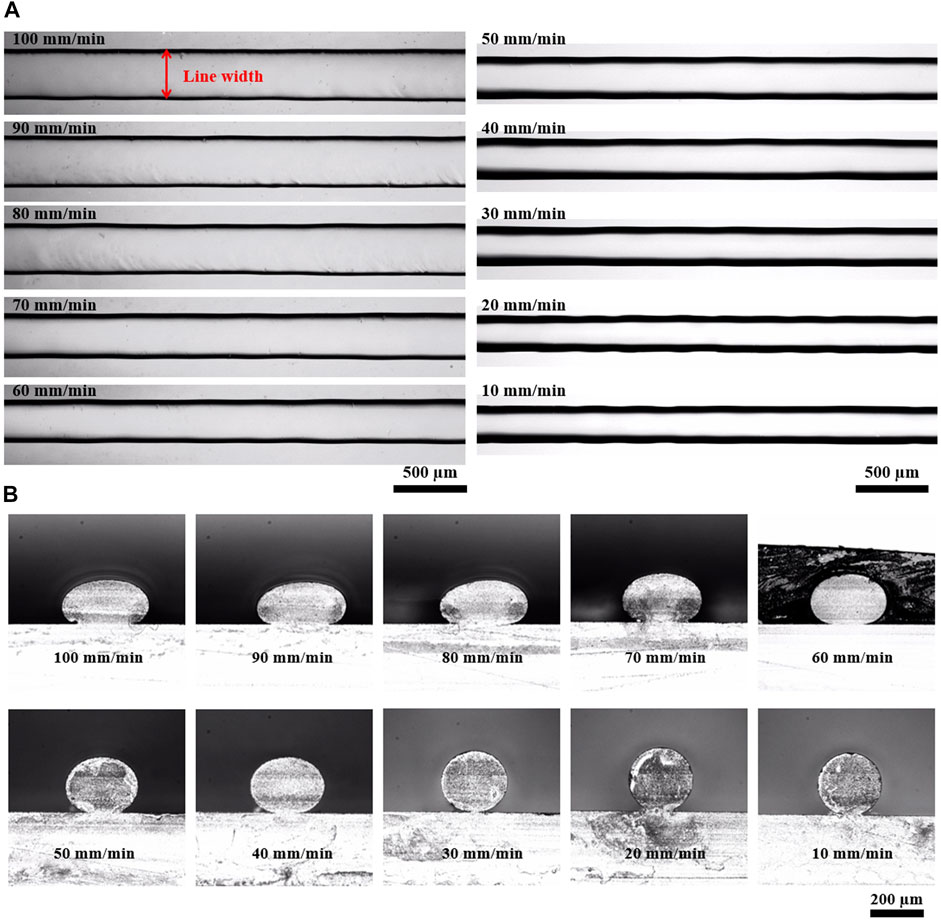
\includegraphics[width=.8\linewidth]{figures/Liu2022_Figure6.jpg}
\caption{Top views and cross-sections of deposited silica lines for travel speeds of 10--100 mm/min and laser powers specified in the original experiment. The figure supports comparison of contact geometry; it is not a generic bubble or residual-stress image. Liu, Oriekhov and Fokine (2022), Figure 6, reproduced unmodified from \href{https://doi.org/10.3389/fmats.2022.978861}{the primary paper} under \href{https://creativecommons.org/licenses/by/4.0/}{CC BY 4.0}.}
\end{figure}
In a simple uniform, plane-stress specimen with fixed principal directions, optical retardation can be written
\begin{equation}
 \delta=C(\lambda,T)(\sigma_1-\sigma_2)d.
\end{equation}
The stress-optic coefficient $C$ is material and wavelength dependent. For a spatially varying field, the interpretation is path dependent; curved surfaces and changing principal directions complicate inversion. SCHOTT describes the relationship between stress birefringence and optical performance.\cite{acad_schott2023} A colorful crossed-polarizer photograph is a useful screening observation, but it is not by itself a calibrated three-dimensional stress map. Darkness can also result from an unfavorable orientation rather than the absence of stress.

This review proposes an acceptance chain tied to intended service: first geometry and surface inspection; then bulk void/inclusion checks; then optical transmission and, where needed, wavefront or haze; then calibrated residual-stress assessment; finally mechanical tests on representative specimens and connections. Hermetic fluidics additionally require pressure and leak testing; decorative lighting requires a different optical specification from an imaging lens. Passing one branch does not certify another. This approach turns the broad word ``transparent'' into measurable requirements while preserving the possibility that intentional texture, color, or scattering is useful product functionality.

\begin{figure}[htbp]\centering
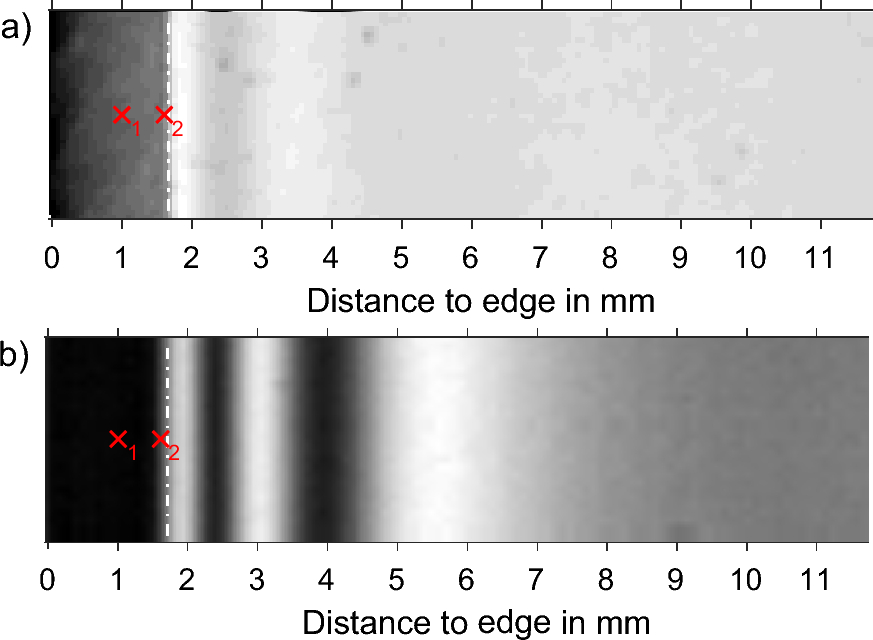
\includegraphics[width=.8\linewidth]{figures/Efferz2024_Figure2.png}
\caption{Measurement-method illustration using conventional fully tempered glass, \emph{not a printed specimen}. Intensity and isochromatic images near the edge of a 10 mm specimen; marked positions are approximately 1.0 and 1.6 mm from the edge, and the dashed line identifies the chamfer. Efferz, Schuler and Siebert (2024), Figure 2, reproduced unmodified from \href{https://doi.org/10.1007/s40940-024-00270-3}{the primary article} under \href{https://creativecommons.org/licenses/by/4.0/}{CC BY 4.0}.}
\end{figure}

\section{Academic landscape and evidence-qualified directory}
\label{sec:directory}
The directory distinguishes demonstrated direct hot-glass deposition from adjacent glass research. Institutional inclusion follows the requested search scope and should not be read as a ranking. A historical project establishes activity at its publication date, not current equipment availability or personnel. ``Not verified'' records a limit of this investigation; it is not proof that a group has never worked on the topic.

\begin{longtable}{P{0.18\textwidth}P{0.22\textwidth}P{0.30\textwidth}P{0.20\textwidth}}
\caption{Global academic research directory. Named people are documented researchers or contacts, not necessarily current laboratory directors. Bibliography entries provide primary DOI/URL links.}\label{tab:academic_directory}\\
\toprule
Institution / laboratory & Researcher / apparatus & Verified contribution and route & Primary reference \\
\midrule
\endfirsthead
\toprule
Institution / laboratory & Researcher / apparatus & Verified contribution and route & Primary reference \\
\midrule
\endhead
MIT Mediated Matter and Glass Lab & Neri Oxman, John Klein, Peter Houk and collaborators; G3DP, G3DP2 & Direct reservoir extrusion; integrated heating and motion; architectural demonstrators. Historical project attribution. & \cite{acad_klein2015,acad_inamura2018} \\
TU Delft structural glass research & Telesilla Bristogianni, Faidra Oikonomopoulou; molten printer name not verified & Cast/recycled structural glass and fabrication research. Casting evidence must not be relabeled as direct AM. & Institutional publication directory \cite{acad_delft} \\
LLNL glass AM / optics & Rebecca Dylla-Spears, Du Nguyen, Joel Destino and collaborators; DIW research systems & Silica and mixed-oxide inks, subsequent thermal densification, optical characterization. Indirect route. & \cite{acad_nguyen2017,acad_destino2018} \\
Fraunhofer IKTS & Glass/ceramic processing teams; specific PI and printer name not verified & Glass-filled filament shaping followed by sintering; photomultiplier-related components. & Institute account \cite{acad_ikts} \\
Fraunhofer ISC with IOF & Project team; specific molten printer not verified & ORMOCER hybrid optical components; inorganic--organic polymer material must be distinguished from glass melt. & Institute account \cite{acad_isc} \\
Fraunhofer IPT & 3DHeat team; metal LPBF and wire deposition tooling & Additively manufactured metal molds with thermal control for glass molding. The tool is printed, not the glass. & 2025--2027 project \cite{acad_ipt} \\
KTH / Nobula & Chunxin Liu, Taras Oriekhov, Michael Fokine; laser filament research printer & Direct fused-silica filament deposition with symmetric heating and measured interlayer bonding. & \cite{acad_liu2022} \\
RISE Acreo with KTH / NTNU & Individual PI/apparatus assignment not verified & Institutional evidence of collaboration in laser processing and glass AM; no separate RISE printer specification inferred. & KTH project record \cite{acad_kthrise} \\
Universit\'e Laval, COPL & Yannick Ledemi, Youn\`es Messaddeq and collaborators; modified commercial extrusion printer & Direct arsenic-sulfide chalcogenide glass deposition. Separate LRIO work addresses nanocomposite photopolymerization. & \cite{acad_baudet2019,acad_lavalproject} \\
McGill University & Inorganic molten-glass PI/apparatus not verified & Search retrieved carbohydrate-glass bioprinting evidence, which is outside this review's inorganic-glass scope. & Repository distinction \cite{acad_mcgill} \\
Nagaoka University of Technology & Historical Takayuki Komatsu glass/crystal research; direct printer not verified & Glass/crystal and laser-processing research provides adjacent expertise; direct molten deposition claim remains unverified. & Institutional record \cite{acad_nagaoka} \\
Laser Zentrum Hannover / Quarzglas-Technologie Heinrich & Philipp von Witzendorff, Leonhard Pohl and collaborators; CO$_2$ deposition head & Direct quartz-fiber deposition using laser heating. & \cite{acad_witzendorff2018} \\
TU Darmstadt / Deakin & Matthias Seel, Nick Birbilis and collaborators; extruded soda-lime specimens & Toolpath-dependent mechanical behavior and four-point bend tests; useful 2026 structural evidence. & \cite{acad_chhadeh2026} \\
\bottomrule
\end{longtable}

\subsection{How to interpret the research network}
The most useful collaboration depends on the missing capability. Reservoir extrusion needs melt conditioning, refractory compatibility, motion coordination, and annealing capacity. Fused-silica filament deposition depends more directly on laser delivery, feedstock uniformity, and local bonding. Optical-quality ink routes instead place substantial demands on colloid formulation, drying, organic removal, densification, and finishing. These categories overlap in characterization but do not share interchangeable processing temperatures or material supply chains.

Two attribution errors deserve explicit correction. First, publication in proceedings hosted at TU Delft does not mean that the printer belongs to TU Delft: the 2024 recycled-glass extrusion study identifies Evenline and MIT authors.\cite{acad_stern2024} Second, the KTH article's affiliations identify KTH and Nobula; its editor's RISE affiliation is not evidence that RISE operated that apparatus. The separate institutional collaboration record establishes RISE involvement at project level, with a narrower evidentiary claim.\cite{acad_liu2022,acad_kthrise}

Laval is a verified direct-glass-extrusion contributor, but its arsenic-sulfide composition belongs to the chalcogenide family and uses a substantially different processing window from silicates.\cite{acad_baudet2019} Its later nanocomposite-resin project is an additional route, not evidence that the chalcogenide platform prints silica.\cite{acad_lavalproject} McGill and Nagaoka remain explicit search gaps for the requested direct molten inorganic-glass directory. Resolving them would require a primary apparatus paper, thesis, patent, or laboratory record identifying both the material and the deposition process; general expertise in glass or additive manufacturing is insufficient.

This evidence structure favors reproducible comparisons and appropriate research partnerships. A prospective collaboration brief should specify composition, size range, required optical function, and final thermal treatment before naming a preferred institution. Such a brief is more informative than a broad list of organizations associated with the phrase ``glass 3D printing.''

\section{Commercial systems, applications, and economics}
\label{sec:commercial}

\subsection{What the available evidence establishes}
The commercial landscape comprises distinct businesses: commissioned molten-glass objects, research printers using locally heated glass filament, and composite materials converted into glass after shaping. Their addressable parts, skill requirements, and qualification burdens differ. Consequently, a vendor list is not a ranking of interchangeable machines. This assessment separates supplier statements, experimentally characterized specimens, patent disclosures, and financial records. Public information was checked on 26 September 2026. No independently audited machine prices, production yields, or application-specific technology readiness levels were established; the qualitative maturity descriptions in Table~\ref{tab:commercial} should not be converted into numerical TRLs.

\begin{table}[htbp]
\centering
\caption{Commercial and industrial landscape. NR means not reported or not verified in the accessed primary sources. Operating temperatures are not maximum equipment ratings.}
\label{tab:commercial}
\scriptsize
\begin{tabularx}{\textwidth}{@{}P{0.14\textwidth}P{0.13\textwidth}P{0.17\textwidth}P{0.15\textwidth}Y@{}}
\toprule
Company / machine & Route & Maximum extrusion temperature & Feedstock & Target market; evidenced maturity \\
\midrule
Evenline / Mark III & Molten extrusion & NR; advertised operation $2000\,^{\circ}\mathrm{F}\approx1093\,^{\circ}\mathrm{C}$ & Studio, container, float glass & Art/design; operating studio platform. Structural masonry remains experimental \cite{com_evenline,com_masonry}. \\
Maple Glass Printing / Maple 4 in 2026 study & Heated-nozzle deposition & NR & Soda-lime rods in study & Research, education, architecture, art; experimental use verified, current sales unverified \cite{com_maple,acad_chhadeh2026}. \\
Nobula / Zero in 2024 study & Laser filament deposition & Current rated maximum NR & Fused-silica filament in study & Micro-optics; characterized research specimens and commercialization programme \cite{com_liu,com_nobulagrant}. \\
Glassomer / materials and parts service & Composite shaping and sintering & Not molten extrusion; room-temperature shaping & Silica--organic composite & Optics, microfluidics, prototypes; supplier materials and component offerings \cite{com_glassomer}. \\
UpNano + Glassomer / NanoOne + UpQuartz & Two-photon polymerization and sintering & Not molten extrusion; $1300\,^{\circ}\mathrm{C}$ sintering & Silica nanocomposite & Precision small parts; vendor process and resin offering \cite{com_upnano}. \\
\bottomrule
\end{tabularx}
\end{table}

\subsection{Company profiles and limits of comparison}
Evenline identifies Michael Stern as its founder and lead \cite{com_evenlinepeople}. Its technology page names Mark III, gives a $325\times325\times380$ mm fabrication envelope, and describes ceramic-nozzle deposition, manual separation of the object from the melt stream, and overnight cooling in a separate chamber. These details make operator involvement and annealer capacity relevant to throughput; the advertised envelope is not a guarantee for every geometry. A vendor process video is available at \href{https://www.evenline.co/technology}{Evenline's technology page}. Neither an equipment price nor a validated maximum extrusion temperature appears in that source \cite{com_evenline}.

The 2024 masonry paper characterizes G3DP3, an Evenline-operated system, and interlocking glass units \cite{com_masonry}. Its academic publication strengthens the evidence beyond photographs, but company-affiliated participation means this is not independent customer acceptance testing. The university account reports that the strongest units combined printed bodies with separately produced interlocking features, and presents larger self-supporting structures as future work \cite{com_mitbricks}. A tested prototype is therefore evidence of architectural potential, not an established building product. Qualification would need to address joints, impact, sustained and lateral loads, statistical variability, and installation details for the intended structure.

Maple remains identifiable through Monash University's venture directory and patent publication AU2021289614A1. The latter lists Nick Birbilis, Darren Robert Feenstra, and Tony Koutsonikolas as inventors and Maple Glass Printing Pty Ltd as applicant/assignee. Its disclosed system heats glass in a nozzle and describes driven solid feedstock; this establishes an invention disclosure, not throughput or machine reliability. Inventorship is not proof of a founding-team role, and the displayed patent-status field is not a legal opinion \cite{com_maple,com_maplepatent}. A 2026 study explicitly identifies Maple 4 and characterizes toolpath-dependent mechanical behavior of printed soda-lime specimens, providing recent experimental evidence \cite{acad_chhadeh2026}. The manufacturer's current website was not successfully verified, so present sales availability, price, and rated temperature ceiling remain unknown.

KTH's programme directory names Michael Fokine, Chunxin Liu, and Taras Oriekhov as Nobula's team. KTH Holding's May 2022 announcement confirms an investment and reports two patent filings, without establishing their subsequent grant status or disclosing investment value \cite{com_nobulateam,com_nobulainvest}. CORDIS verifies an EU contribution of EUR~2,499,875 for project 190122644, with total project cost EUR~3,571,250 and an end date of 30 April 2026. These are project-finance figures, not printer prices or cumulative company funding. Its product-performance language belongs to the project description and requires separate validation \cite{com_nobulagrant}.

Liu and colleagues used Nobula Zero to make fused-silica microlens arrays, with 200~$\mu$m filament and a CO$_2$ laser. Their study demonstrates a particular optical manufacturing workflow, including laser postprocessing; it cannot establish that every glass part requires no finishing. Several authors have Nobula affiliations. Supplier descriptions and this research should therefore be labelled separately, without calling either independent validation of a complete product range \cite{com_liu}. The live 2026 website confirms the company's laser-based manufacturing direction but did not expose a numerical specification table in the accessible page; current sales configuration, acceptance criteria, and price remain procurement questions \cite{com_nobula}.

Glassomer's history records its formation in Karlsruhe in 2018 and subsequent move to Freiburg. Its current offering includes composite materials, prototyping, and fused-silica components; this is a materials/process business rather than a like-for-like molten extrusion machine \cite{com_glassomerhistory,com_glassomer}. The UpNano collaboration extends the route to NanoOne two-photon polymerization using UpQuartz. Its 2024 manufacturer announcement specifies binder removal at $600\,^{\circ}\mathrm{C}$, sintering at $1300\,^{\circ}\mathrm{C}$, and approximately 30\% isotropic shrinkage. Those values apply to that reported material/process, not all Glassomer formulations. Published demonstrations include ferrules and a small filter, supporting precision-part targeting while leaving production yield unreported \cite{com_upnano}.

\subsection{Application fit and competitive alternatives}
The strongest near-term case for large molten beads is custom shape and visible material expression. Art, lighting, and limited-run packaging concepts can accept a layered surface when it is part of the design. Functional packaging adds closure tolerances, cleanability, impact resistance, and repeatability; an attractive vessel alone does not establish suitability for food, pharmaceuticals, or pressurization. Structural masonry is supported by specimen and assembly research, while broad architectural deployment remains an inference requiring application testing \cite{com_masonry}.

For lenses, optical channels, and chemical microdevices, high value per part can justify slower fabrication and metrology. Laser filament deposition has direct micro-optical evidence, and composite routes have supplier offerings in optics and microfluidics \cite{com_liu,com_glassomer}. Nevertheless, hermetic chemical vessels require verified leak tightness, pressure capability, connection integrity, and chemical compatibility for the actual fluid and temperature. Radioactive-waste vitrification containers are treated here as a proposed research direction: this source set establishes neither a qualified printed containment product nor a commercial deployment. Glass chemistry and a printable shape are insufficient evidence of long-term containment performance.

Conventional alternatives remain the baseline for purchasing decisions. Blowing and lampworking offer skilled manipulation of hollow forms; casting spreads tooling and furnace costs over repeated parts; machining and polishing support controlled surfaces on suitable blanks. Indirect AM introduces binder removal, shrinkage compensation, and sintering, whereas molten deposition transfers difficulty into thermal control, bead geometry, and annealing. These process differences motivate a matched-part comparison: identical composition or function, dimensional tolerances, inspected surface area, accepted yield, and annual volume. Comparing a millimetre optical component with a kilogram decorative print on cost per kilogram would conceal the product value and the inspection burden.

\subsection{Transparent cost model and illustrative sensitivities}
No supplier quotation is fabricated here. A reproducible planning model expresses cost per accepted part as
\begin{equation}
 C_{\mathrm{good}}=\frac{K/Y+F}{N_a y}
 +\frac{m c_m+E c_e+t_l c_l+c_q+c_p}{y},
\label{eq:commercialcost}
\end{equation}
where $K$ is installed capital, $Y$ depreciation life in years, $F$ annual fixed cost, $N_a$ annual attempted parts, and $y$ accepted yield. The remaining terms represent charged feedstock, electricity, labour, inspection, and consumables/postprocessing per attempt. All costs must share a currency and price basis. This simplified straight-line model excludes financing, taxes, residual value, and schedule-dependent rework; late failures are assumed to consume a full attempt. Parallel printer and annealer schedules must be checked before assuming $N_a$ is achievable.

For an explicitly hypothetical studio cell, let $K=\$100{,}000$, $Y=5$, $F=\$10{,}000$/year, $N_a=1000$, and $y=0.80$. Assume 2 kg of charged feedstock at \$2/kg, 20 kWh at \$0.15/kWh, one labour hour at \$30/h, \$10 inspection, and \$5 consumables per attempt. Annual fixed cost is \$30,000 and variable cost \$52/attempt, giving \$102.50/accepted part. These analyst-selected values are neither a price estimate for Evenline nor measured energy consumption. At 250 attempts/year, the same arithmetic gives \$215.00; at 2000 it gives \$83.75. At the baseline volume, lowering yield to 0.60 raises cost to \$136.67. Doubling electricity price raises baseline cost only to \$106.25 under these assumptions.

A second hypothetical small-part indirect-AM cell assumes $K=\$60{,}000$, $Y=5$, $F=\$6000$/year, $N_a=2000$, and $y=0.90$. Per attempt, allocate \$5 resin, 2 kWh at \$0.15/kWh, 0.25 labour hours at \$30/h, \$3 inspection, and \$2 firing consumables. The result is \$29.78/accepted part. This is not a finding that indirect AM is cheaper: the illustrative product is smaller, furnace energy is a batch allocation, and geometric acceptance may differ. Underfilled firing batches or additional optical polishing can reverse a superficial comparison. A useful quotation request therefore specifies the actual part, allowable defects, batch size, annual demand, training, furnace installation, maintenance, spare nozzles or optics, and acceptance tests. Until such matched quotations and meter readings exist, utilization and yield sensitivities are more defensible than a claimed market-wide CapEx or OpEx ranking.

\section{Open frontiers and a research roadmap}
\label{sec:roadmap}
\subsection{Prioritize a repeatable process window}
The reviewed work establishes a range of feasible geometries and material routes. The next useful step is a repeatable, application-specific process window linking feedstock, thermal history, deposition geometry, and accepted properties. This section proposes an experimental programme; its milestones are recommendations rather than reported achievements.

Begin with a single documented glass composition and a representative part family. Obtain chemical identity and thermal reference data, then measure deposited mass and bead geometry over controlled combinations of temperature, head or feed rate, travel speed, and layer return time. Preserve both successful and failed runs. A process window containing only attractive parts cannot identify failure boundaries or predict yield.

\begin{longtable}{@{}P{.18\textwidth}P{.34\textwidth}P{.39\textwidth}@{}}
\caption{Proposed staged research programme. Progression depends on evidence rather than an arbitrary calendar.}\label{tab:roadmap}\\
\toprule Stage & Experiment and recorded variables & Evidence required to progress \\
\midrule\endfirsthead
\toprule Stage & Experiment and recorded variables & Evidence required to progress \\
\midrule\endhead
Feedstock baseline & Named batch; chemistry, moisture/contamination, viscosity anchors, thermal expansion; inspect rods or cullet & Traceable batch identity; justified temperature window; baseline specimen properties \\
Single-track map & Gravimetric flow, actual temperatures, head/feed, speed, gap, width, height, contact width & Repeatability distributions and failure boundaries; quantified restart and corner behavior \\
Thermal qualification & Thick-section surrogate, layer revisit time, calibrated pyrometry, chamber/part offsets & Verified stress reduction without unacceptable slumping; internal temperature model checked against data \\
Interface and defect study & Controlled orientation and thermal history; sectioning, microscopy, CT where resolution allows, bend/fracture tests & Failure origins correlated with material/process variables; distinguish lack of contact from intrinsic glass fracture \\
Representative parts & Geometry and functional tolerances, optical tests or pressure/leak tests, full thermal cycle & Predeclared acceptance criteria; documented yield, cycle time and metrology repeatability \\
Production comparison & Matched-part blowing/casting/machining/indirect AM benchmarks, energy meters, labor and maintenance logs & Cost per accepted part with utilization sensitivity; no conversion of nominal deposition rate into production capacity \\
\bottomrule\end{longtable}

\subsection{Measurements that could change engineering decisions}
\textbf{Closed-loop deposition.} The controller should distinguish sensor validity from control performance. Glass transparency, emissivity variation, hot background reflections, and laser interference can bias a thermal reading. Validate a sensing arrangement before tuning control gains, and evaluate unseen geometries rather than only training trajectories. Published quartz-glass temperature feedback provides a concrete starting point, with apparatus-specific calibration still necessary.\cite{acad_chen2025}

\textbf{Toolpath and thermal memory.} Direction, speed, and return time are coupled. The 2026 toolpath study supports testing orientation and retained heat together, while also illustrating why a within-study strength improvement should not be converted directly into a structural design factor. A factorial or response-surface programme should record the physical path and interface temperature rather than just a slicer orientation label.\cite{acad_chhadeh2026}

\textbf{Recycled feedstock.} Sorting and conditioning are upstream process controls. A comparison should separate a known single-source cullet stream from mixed unknown glass. Quantify batch variation, contamination introduced during grinding or handling, and the fraction rejected before printing. Recycled-glass demonstrators establish feasibility; closed-loop recycling and environmental benefit require additional mass and energy accounting.\cite{acad_stern2024}

\textbf{Optical and structural function.} Freeform illumination, micro-optics, chemical channels, and masonry connections demand different validation. High transmission does not establish a low wavefront error; compression testing of a brick does not establish impact resistance or connection durability. Application-specific acceptance is the mechanism by which a research demonstrator becomes a credible product.

\subsection{An intellectual-property and demonstration map}
Three downloaded disclosures complement the apparatus literature: MIT's \href{https://patents.google.com/patent/US10266442B2/en}{US10266442B2}, Maple's \href{https://patents.google.com/patent/AU2021289614A1/en}{AU2021289614A1}, and LLNL's \href{https://patents.google.com/patent/WO2020118157A1/en}{WO2020118157A1}. They concern different aspects of glass manufacture and feedstock. Patent descriptions and illustrations provide engineering concepts; they do not demonstrate commercial availability, achieved accuracy, or validated lifetime. This review performs no freedom-to-operate analysis or legal-status certification.

The \href{https://www.media.mit.edu/projects/g3p/overview/}{MIT Glass I project page} and \href{https://www.evenline.co/technology}{Evenline technology demonstrations} provide visual process context. The asset ledger retains direct streaming links where established. An HTTP response confirms accessibility at the request time, not successful playback or the authenticity of every quantitative claim in a video. The supplied media notes identify provenance and reproduction terms separately from scientific interpretation.

\subsection{Reproducibility and remaining evidence gaps}
Direct demonstration links retained in the asset ledger are \href{https://vimeo.com/136764796}{MIT Glass I / G3DP}, \href{https://vimeo.com/211778198}{MIT Glass II / G3DP2}, and \href{https://www.youtube.com/watch?v=CSw0Kw6M8i0}{Inside Maple Glass Printing}. The \href{https://www.memphis.edu/physics/demonstrations/polariscope.php}{University of Memphis polariscope page} links a \href{https://www.youtube.com/watch?v=IefRrdTmlbA}{direct educational demonstration}. These links were checked for HTTP accessibility; playback was not verified. The polariscope video is not claimed to show a printed-glass specimen.

The analysis scripts regenerate nominal viscosity fits, residual plots, flow sensitivity, thermal scales, and the commercial scenarios. The viscosity thresholds CSV records extrapolation flags. All calculations use explicit inputs and are distinct from experimentally measured machine output. The complete LaTeX project permits updating a figure, source, or chapter without replacing the underlying evidence trail.

Important gaps remain: matched-route tensile datasets; wavelength-, thickness-, and surface-controlled optical comparisons; independently audited current printer prices and yields; material-specific refractory lifetime; and verified direct molten-silicate apparatus attribution for some requested institutions. These are limits of the evidence base, not blanks filled with estimates. Future updates should add new primary measurements and revise the corresponding decision, rather than merely extend a list of references.

The practical recommendation is to choose a material route from the required final function. Use reservoir extrusion where large continuous forms and layer texture are compatible with the product; investigate laser filament deposition where local heating and small features are valuable; evaluate indirect routes where fine geometry and densification can be qualified. In each case, measure the complete path to an accepted part, including finishing and thermal treatment.

\clearpage
\begingroup
\RaggedRight
\bibliographystyle{plainnat}
\bibliography{references}
\endgroup
\end{document}
